%{\color{red} 
%- how does OS manage memory\\
%- page tablesi and hugepages (take it from Jeff's paper)\\
%- GPU page tables\\
%- how does migration happen\\
%- GPU programming and CUDA\\
%}
%
Systems using heterogeneous CPU and GPU computing resources have been widely
used for several years.
%Until recently, the GPU has been managed as a separate
%accelerator, requiring explicit memory management by the programmer to transfer
%data to and from the GPU's address space and (typically) the GPU's
%locally-attached memory.  To increase programmer productivity and broaden the
%classes of workloads that the GPU can execute, recent systems have introduced
%automatic memory management enabling the CPU and GPU to access a unified address
%space and transparently migrate data at a page-level granularity~\cite{UVM}.
%The next step in this evolution is making the GPU a cache-coherent peer to the
%CPU in the memory system, which is the stated goal of a number of commercial
%vendors~\cite{HSA}.
High performance GPUs have developed into stand-alone PCIe-attached
accelerators requiring explicit memory management by the programmer to control
data transfers into the GPU's high-bandwidth locally attached memory. As GPUs
have evolved, the onus of explicit memory management has been addressed by
providing a unified shared memory address space between the GPU and
CPU~\cite{UVM,HSA}.  Whereas a single unified virtual address space improves
programmer productivity, discrete GPU and CPU systems still have separate
locally attached physical memories, optimized for bandwidth and latency
respectively. 


\begin{figure}[t]
    \centering
    \subfloat[Bandwidth sensitivity] {
        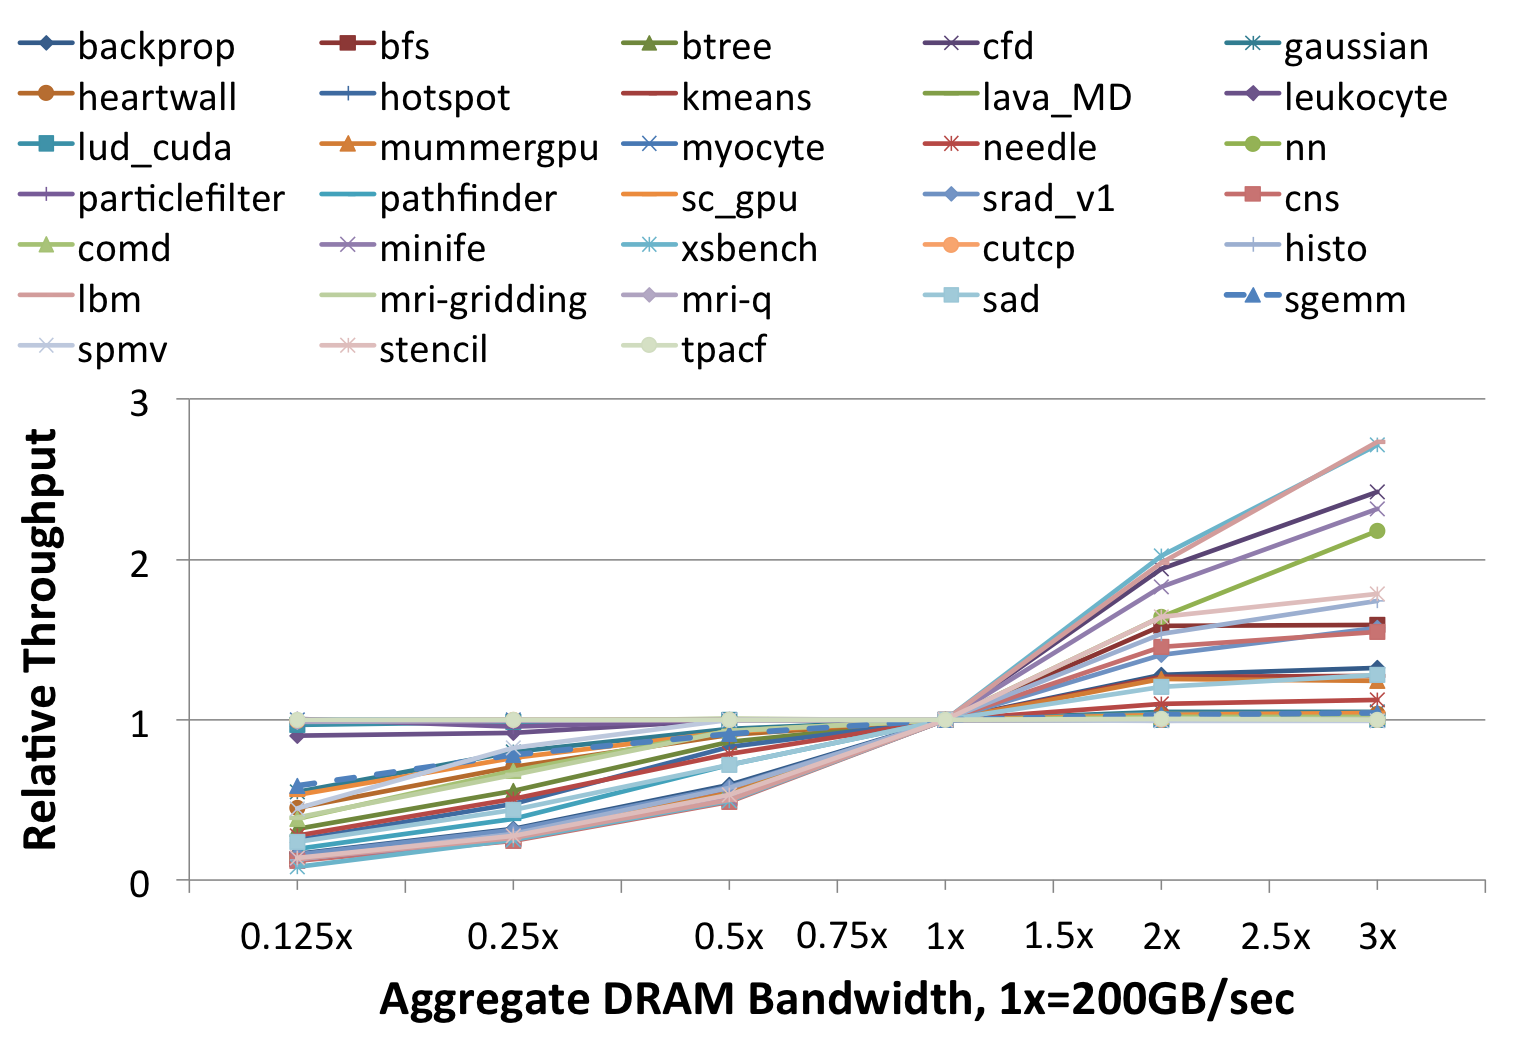
\includegraphics[width=0.7\columnwidth]{asplos2015/figures/bandwidth-1.png}
        \label{fig:bandwidth}
    }
    \\
    \subfloat[Latency sensitivity] {
        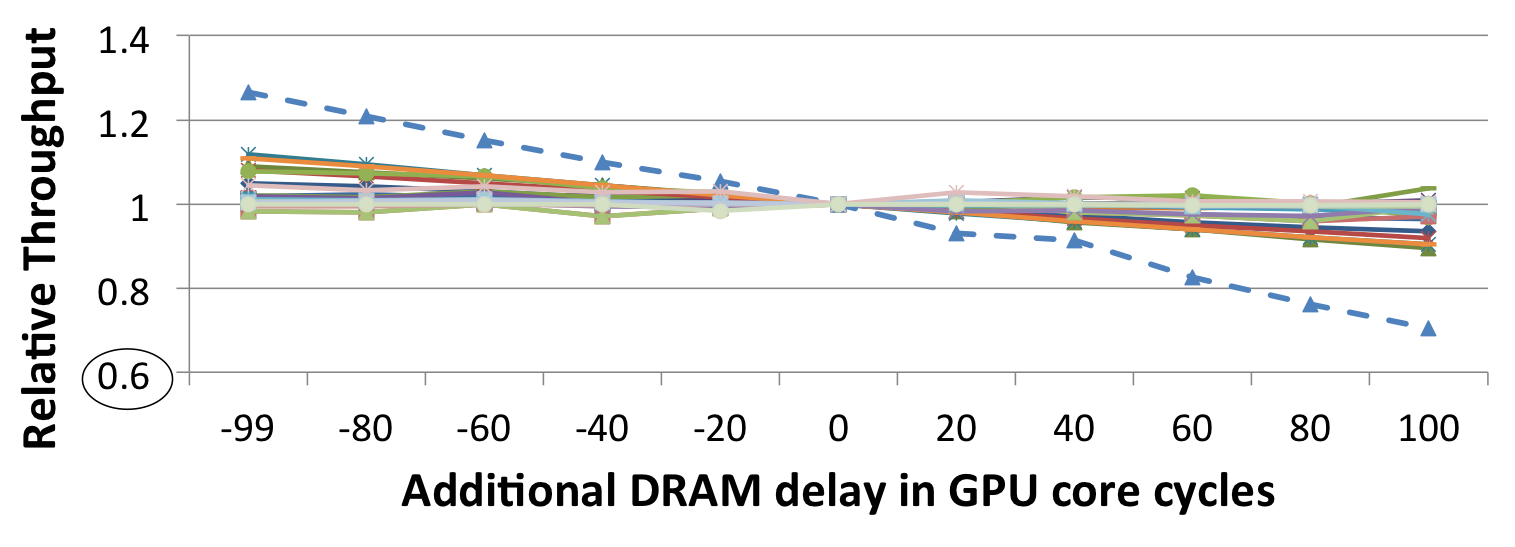
\includegraphics[width=0.7\columnwidth]{asplos2015/figures/latency-1.png}
        \label{fig:latency}
    }
    \caption{GPU performance sensitivity to bandwidth and latency changes.}
    \label{fig:bwlatencysensitivity}
\end{figure}

\section{Bandwidth Hungry Characteristics of GPUs}
%\subsection{{Heterogeneous CC-NUMA Systems}}
\label{heterogeneous_background}
%While some heterogeneous CPU/GPU systems share a single unified physical
%memory~\cite{AMDAPU}, discrete GPUs are already using specialized DRAM optimized
%to meet their high bandwidth demands.
A by-product of the GPU's many-threaded design is that it is able to maintain a
large number of in-flight memory requests and execution throughput is correlated
to memory bandwidth rather than latency, as compared to CPU designs.  As a
result, GPUs have chosen to integrate high bandwidth off-package memory like
GDDR rather than accessing the CPU's DDR directly or integrating DDR locally on
the GPU board. 

To highlight the sensitivity of GPU performance to memory characteristics,
Figures~\ref{fig:bandwidth} and~\ref{fig:latency} show the performance variation
as memory bandwidth and latency vary for a variety of GPU compute benchmarks
from the Rodinia~\cite{Che2009} and {\color{black}Parboil~\cite{Parboil} suites,
as well as a number of recent HPC~\cite{comd,cns,minife,xsbench} workloads. Most
of these GPU workloads are sensitive to changes in bandwidth, while showing much
more modest sensitivity to varying the latency; only {\tt sgemm} stands out as
highly latency sensitive among these 33 workloads. Some application kernels are
neither bandwidth nor latency sensitive and do not see significant performance
variation as modifications are made to the memory subsystem.} While GPU-equipped
systems generally require bandwidth-optimized memories to achieve peak
performance, these memory technologies have significant cost, capacity, and/or
energy disadvantages over alternative DRAM technologies.

The most common Bandwidth-Optimized (BO) memory technology today is
GDDR5~\cite{GDDR5}.  Providing a per-pin data rate of up to 7Gbps, this memory
technology is widely used with discrete GPUs used in HPC, workstation, and
desktop systems.  Due to the high data rates, GDDR5 systems require significant
energy per access and are unable to support high-capacity multi-rank systems.
In contrast, the roadmap for the next several years of cost/capacity-optimized
(CO) DRAM (DDR4 and LPDDR4) provides a per-pin data rate that reaches only 3.2
Gbps.  However, these CO DRAM technologies provide similar latency at a fraction
of the cost and lower energy per access compared to the BO GDDR5 memories.
Looking forward, systems requiring more bandwidth and/or reduced energy per
access are moving to  die-stacked DRAM technologies~\cite{HBM,WIDEIO2}.  These
bandwidth-optimized stacked memories are significantly more energy-efficient
than off-package memory technologies like GDDR5, DDR4, and LPDDR4.
Unfortunately, the number of DRAM die that can be economically stacked in a
single package is limited, necessitating systems to also provide a pool of
off-package capacity-optimized DRAM.

This disaggregation of memory into on-package and off-package pools is one
factor motivating the need to revisit page placement within the context of GPU
performance.  Future GPU/CPU systems are likely to take this disaggregation
further and move capacity-optimized memory not just off the GPU package, but
across a high speed interconnect where it is physically attached to the CPU
rather than the GPU, or possibly further~\cite{Lim2009}.  In a CC-NUMA
system, the physical location of this capacity-optimized memory only changes the
latency and bandwidth properties of this memory pool -- it is functionally
equivalent regardless of being CPU or GPU locally attached.  A robust page
placement policy for GPUs will abstract the on-package, off-package, and remote
memory properties into performance and power characteristics based on which it
can make optimized decisions.

\section{Current OS NUMA Page Placement}
\label{linux_background}
%\vspace{-0.05in}
In modern symmetric multiprocessor (SMP) systems, each socket typically consists
of several {\color{black}cores} within a chip multi-processor (CMP) that share
last-level caches and on-chip memory controllers~\cite{INTELXEON}. The number of
memory channels connected to a processor socket is often limited by the
available pin count.  To increase the available memory bandwidth and capacity in
a system, individual sockets can be connected via a cache coherent interconnect
fabric such as Intel's Quick Path~\cite{INTELQPI}, AMD's
HyperTransport~\cite{AMDHT}, or NVIDIA's NVLink~\cite{NVLINK}.  A single socket,
the processors within it, and the physically attached memory comprise what an
operating system sees as a local NUMA zone.  Each socket is a separate NUMA
zone. While a processor within any given zone can access the DRAM within any
other zone, there is additional latency to service this memory request compared
to a locally serviced memory request because the request must be routed first to
its own memory controller, across the socket interconnect, and through the
remote memory controller.

Operating systems such as Linux have recognized that, unless necessary, it is
typically better for applications to service memory requests from their own NUMA
zone to minimize memory latency.  To get the best performance out of these NUMA
systems, Linux learns system topology information from the Advanced
Configuration and Power Interface (ACPI) System Resource Affinity Table (SRAT)
and memory latency information from the ACPI System Locality Information Table
(SLIT)\@. After discovering this information, Linux provides two basic page
placement policies that can be specified by applications to indicate where they
prefer their physical memory pages to be placed when using standard {\tt malloc}
and {\tt mmap} calls to allocate memory.

\emph{LOCAL:} The default policy inherited by user processes is \emph{LOCAL} in
which physical page allocations will be from memory within the local NUMA zone
of the executing process, unless otherwise specified or due to capacity
limitations.  This typically results in allocations from memory physically
attached to the CPU on which the process is running, thus minimizing memory
access latency.

\emph{INTERLEAVE:} The second available allocation policy, which processes must
specifically inform the OS they would like to use, is \emph{INTERLEAVE}\@. This
policy allocates pages round-robin across all (or a subset) of the NUMA zones
within the SMP system to balance bandwidth across the memory pools.  The
downside of this policy is that the additional bandwidth comes at the expense of
increased memory latency. Today, the OS has no knowledge about the relative
bandwidth of memories in these different NUMA zones because SMP systems have
traditionally had bandwidth-symmetric memory systems.

In addition to these OS placement policies, Linux provides a library interface
called \textit{libNUMA} for applications to request memory allocations from
specific NUMA zones.  This facility provides low-level control over memory
placement but requires careful programming because applications running on
different systems will often have different NUMA-zone layouts.  Additional
difficulties arise because there is no performance feedback mechanism available
to programmers when making memory placement decisions, nor are they aware of
which processor(s) their application will be running on while writing their
application.

With the advent of heterogeneous memory systems, the assumptions that operating
system NUMA zones will be symmetric in bandwidth and power
characteristics break down.  The addition of heterogeneous GPU and CPU computing
resources further stresses the page placement policies since processes may not
necessarily be migrated to help mitigate performance imbalance, as certain
phases of computation are now pinned to the type of processor executing the
program.  As a result, data placement policies combined with
bandwidth-asymmetric memories can have significant impact on GPU, and possibly
CPU, performance.

\begin{figure}[t]
    \centering
    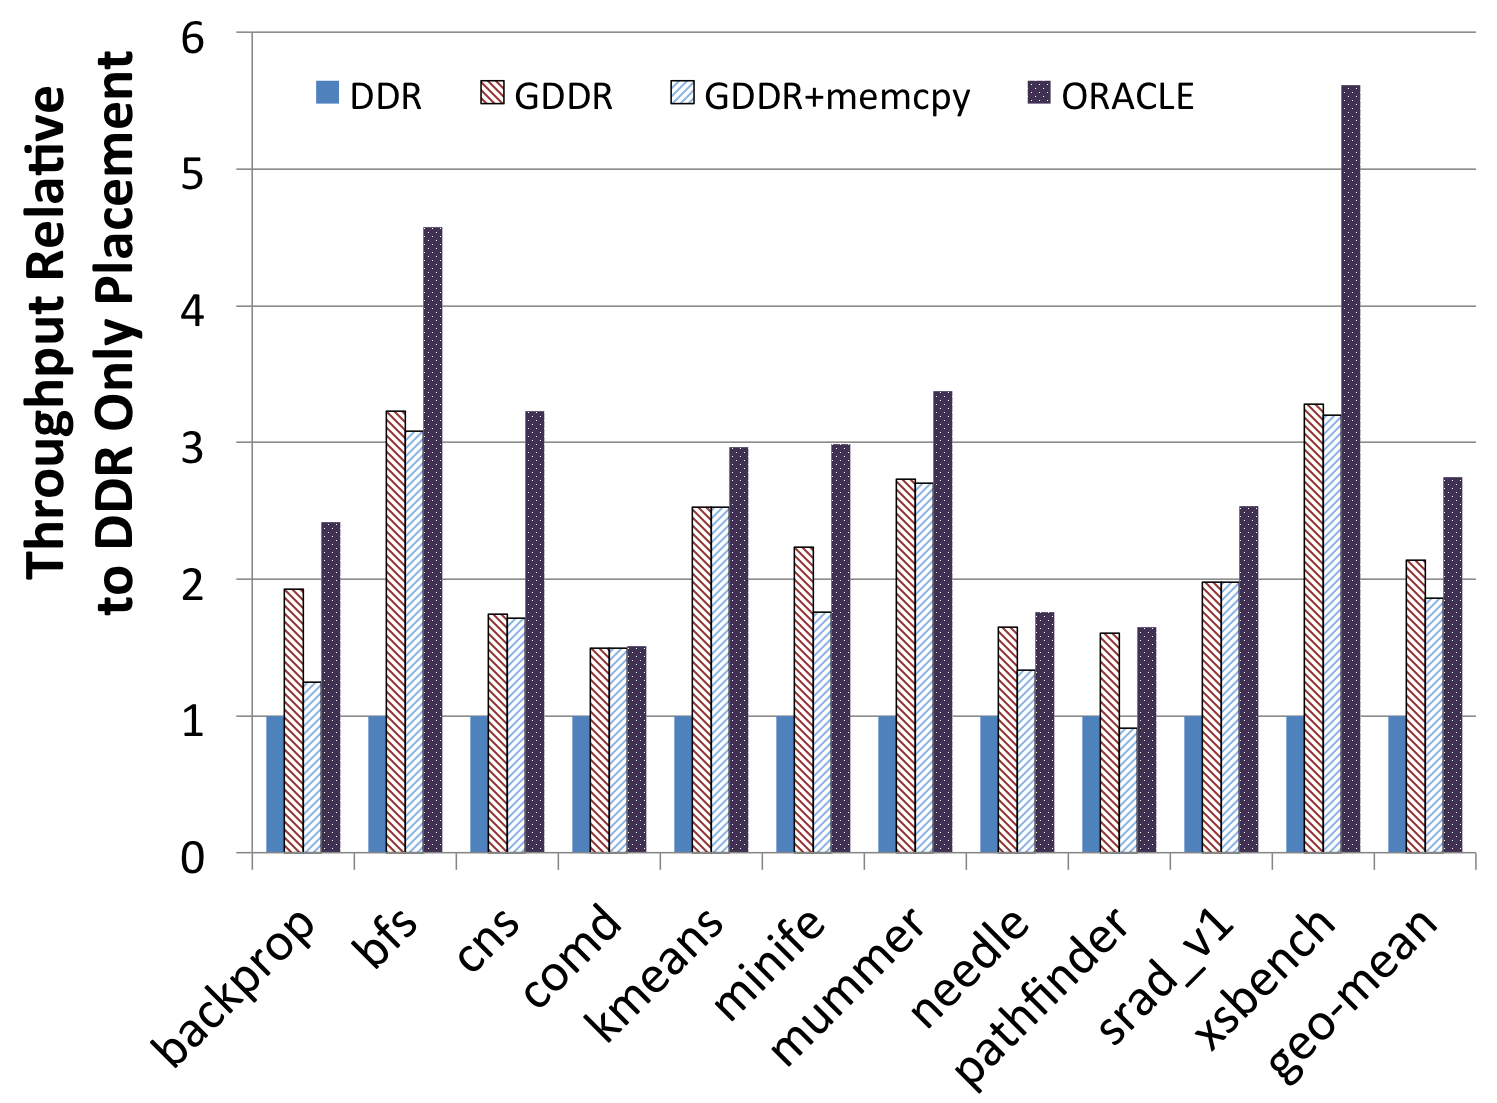
\includegraphics[width=0.7\columnwidth]{hpca2015/figures/motivation.png}
    \caption{GPU performance sensitivity to memory subsystem performance where GDDR provides 
    200GB/s, DDR provides 80GB/s, and {\tt memcpy} bandwidth is 80GB/s.}
    \label{fig:motivation-hpca2015}
\end{figure}

%A by-product of the GPU's many-threaded design is that it is able to maintain a
%large number of in-flight memory requests and execution throughput is correlated
%to memory bandwidth rather than latency, as compared to CPU designs.  As a
%result, GPUs have chosen to integrate high bandwidth off-package memory like
%GDDR rather than accessing the CPU's DDR directly or integrating DDR locally on
%the GPU board.  This choice is motivated by our observation that the performance
%of some GPU compute workloads would degrade by as much as 66\% if the
%traditional GDDR memory on a GPU were replaced with standard DDR memory, as seen
%in Figure~\ref{fig:motivation}.

\section{Memory Copy Overhead in GPUs}
In current CPU/GPU designs, GPU and CPU memory systems are private and require
explicit copying to the GPU before the application can execute.
Figure~\ref{fig:motivation-hpca2015} shows the effect of this copy overhead on
application performance by comparing GDDR to GDDR+{\tt memcpy} performance which
includes the cost of the programmer manually copying data from the DDR to the
GDDR before launching the GPU kernels.  While this copy overhead varies from
application to application, it can be a non-trivial performance overhead for
short-running GPU applications and can even negate the effectiveness of using
the high bandwidth GDDR on-board the GPU in a limited number of cases.

While it is technically possible for the GPU to access CPU memory directly over
PCIe today, the long latency (microseconds) of the access makes this a rarely
used memory operation.  Programming system advancements enabling a uniform
global address space, like those introduced in CUDA 6.0~\cite{cuda}, relax the
requirement forcing programmers to allocate and explicitly copy memory to the
GPU up-front, but do nothing to improve the overhead of this data transfer.
Further, by copying pages from the CPU to the GPU piece-meal on demand, these
new runtimes often introduce additional overhead compared to performing a highly
optimized bulk transfer of all the data that the GPU will need during execution.
The next step in the evolution of GPUs, given the unified addressing, is to
optimize the performance of this new programming model. 

\section {Cache Coherent GPUs Enhancing System Programmability}
\label{chap:background:cc-enhances-programmability}
The key advancement expected to enable performance is the introduction of
CC-NUMA GPU and CPU systems.  Using cache coherence layered upon NVLink, HT, or
QPI, GPUs will likely be able to access CPU memory in hundreds of nanoseconds at
bandwidths up to 128GB/s by bringing cache lines directly into GPU caches.
Figure~\ref{fig:motivation-hpca2015} shows the upper bound (labeled ORACLE) on
performance that could be achieved if both the system DDR memory and GPU GDDR
memory were used concurrently, assuming data had been optimally placed in both
technologies.  In this work, we define oracle placement to be \emph{a priori}
page placement in the GPU memory (thus requiring no migration), of the minimum
number of pages, when sorted from hottest to coldest, such that the GDDR
bandwidth is fully subscribed during application execution.

Because initial CPU/GPU CC-NUMA systems are likely to use a form of IOMMU
address translation services for walking the OS page tables within the GPU,  it
is unlikely that GPUs will be able to directly allocate and map their own
physical memory without a call back to the CPU and operating system.  In this
work, we make a baseline assumption that all physically allocated pages are
initially allocated in the CPU memory and only the operating system or GPU
runtime system executing on the host can initiate page migrations to the GPU\@.
In such a system, two clear performance goals become evident.  The first is to
design a memory policy that balances CC-NUMA access and page migration to simply
achieve the performance of the legacy bulk copy interface without the
programming limitations.  The second, more ambitious, goal is to exceed this
performance and approach the oracular performance by using these memory zones
concurrently, enabling a peak memory bandwidth that is the sum of the two zones.

Achieving either of these goals requires migrating enough data to the GPU to
exploit its high memory bandwidth while avoiding migrating pages that may never
be accessed again.  Every page migration increases the total bandwidth
requirement of the application and over-migration potentially reduces
application performance if sufficient bandwidth headroom in both the DDR and
GDDR is not available.  Thus, the runtime system must be selective about which
pages to migrate.  The runtime system also must be cognizant that performing TLB
invalidations (an integral part of page migration) on a GPU does not just halt a
single processor, but thousands of compute pipelines that may be accessing these
pages through a large shared TLB structure.  This shared TLB structure makes
page migrations between a CPU and GPU potentially much more costly (in terms of
the opportunity cost of lost execution throughput) than in CPU-only systems.

In addition to managing the memory bandwidth overhead of page migration and
execution stalls due to TLB shootdowns, the relative bandwidth utilization of
both the CPU and GPU memory must be taken into account when making page
migration decisions.  When trying to balance memory bandwidth between two
distinct memory zones, it is possible to over- or under-subscribe either memory
zone. Migrating pages too slowly to the GPU memory will leave its local memory
sitting idle, wasting precious bandwidth.  Conversely, migrating pages to the
GPU too aggressively may result in under-utilization of the CPU memory while
paying the maximum cost in terms of migration overheads. A comprehensive CPU-GPU
memory management solution will attempt to balance all of these effects to
maximize memory system and GPU throughput in future mobile, graphics, HPC, and
data-center installations.

\section{Supporting Hardware Cache Coherence in GPUs}
\label{chap:background:hw-cc-is-hard}
%Heterogeneous CPU--GPU systems have been widely adopted by the high performance
%computing community and are becoming increasingly common in other computing
%paradigms. High performance GPUs have developed into stand-alone PCIe-attached
%accelerators requiring explicit memory management by the programmer to control
%data transfers into the GPU's high-bandwidth locally attached memory. As GPUs
%have evolved, the onus of explicit memory management has been addressed by
%providing a unified shared memory address space between the GPU and
%CPU~\cite{UVM,HSA}.  Whereas a single unified virtual address space improves
%programmer productivity, discrete GPU and CPU systems still have separate
%locally attached physical memories, optimized for bandwidth and latency
%respectively. 

Managing the physical location of data, and guaranteeing that reads access the
most up-to-date copies of data in a unified shared memory can be done through
the use of page level migration and protection. Such mechanisms move data at the
OS page granularity between physical memories~\cite{UVM}.  With the advent of
non-PCIe high bandwidth, low latency CPU--GPU interconnects, the possibility of
performing cache-line, rather than OS-page-granularity, accesses becomes
feasible.  Without OS level page protection mechanisms to support correctness
guarantees, however,  the responsibility of coherence has typically fallen on
hardware cache-coherence implementations.

\begin{table}[t]
\begin{center}
\begin{tabular}{ddd}
 \hline
 \multicolumn{1}{l}{Workload} &   \multicolumn{1}{c}{L1 Hit Rate (\%)}  &  \multicolumn{1}{c}{L2 Hit Rate (\%)}  \\
 \hline
 \hline
 \multicolumn{1}{l}{backprop}  &   62.4  &   70.0\\
 \hline
 \multicolumn{1}{l}{bfs}  &   19.6  &   58.6  \\
 \hline
 \multicolumn{1}{l}{btree}  &   81.8  &   61.8  \\
 \hline
 \multicolumn{1}{l}{cns}  &   47.0  &   55.2  \\
 \hline
 \multicolumn{1}{l}{comd}  &   62.5  &   97.1  \\
 \hline
 \multicolumn{1}{l}{kmeans}  &   5.6  &   29.5  \\
 \hline
 \multicolumn{1}{l}{minife}  &   46.7  &   20.4  \\
 \hline
 \multicolumn{1}{l}{mummer}  &   60.0  &   30.0  \\
 \hline
 \multicolumn{1}{l}{needle}  &   7.0  &   55.7  \\
 \hline
 \multicolumn{1}{l}{pathfinder}  &   42.4  &   23.0  \\
 \hline
 \multicolumn{1}{l}{srad\_v1}  &   46.9  &   25.9  \\
 \hline
 \multicolumn{1}{l}{xsbench}  &   30.7  &   63.0  \\
 \hline
 \hline
 \multicolumn{1}{l}{Arith Mean}  &   44.4  &   51.6  \\
\hline
\end{tabular}
\caption{GPU L1 and L2 cache hit rates (average).}
\label{tab:gpuhitrate}
\end{center}
\vspace{-.25in}
\end{table}

\begin{figure*}[t]
    \centering
    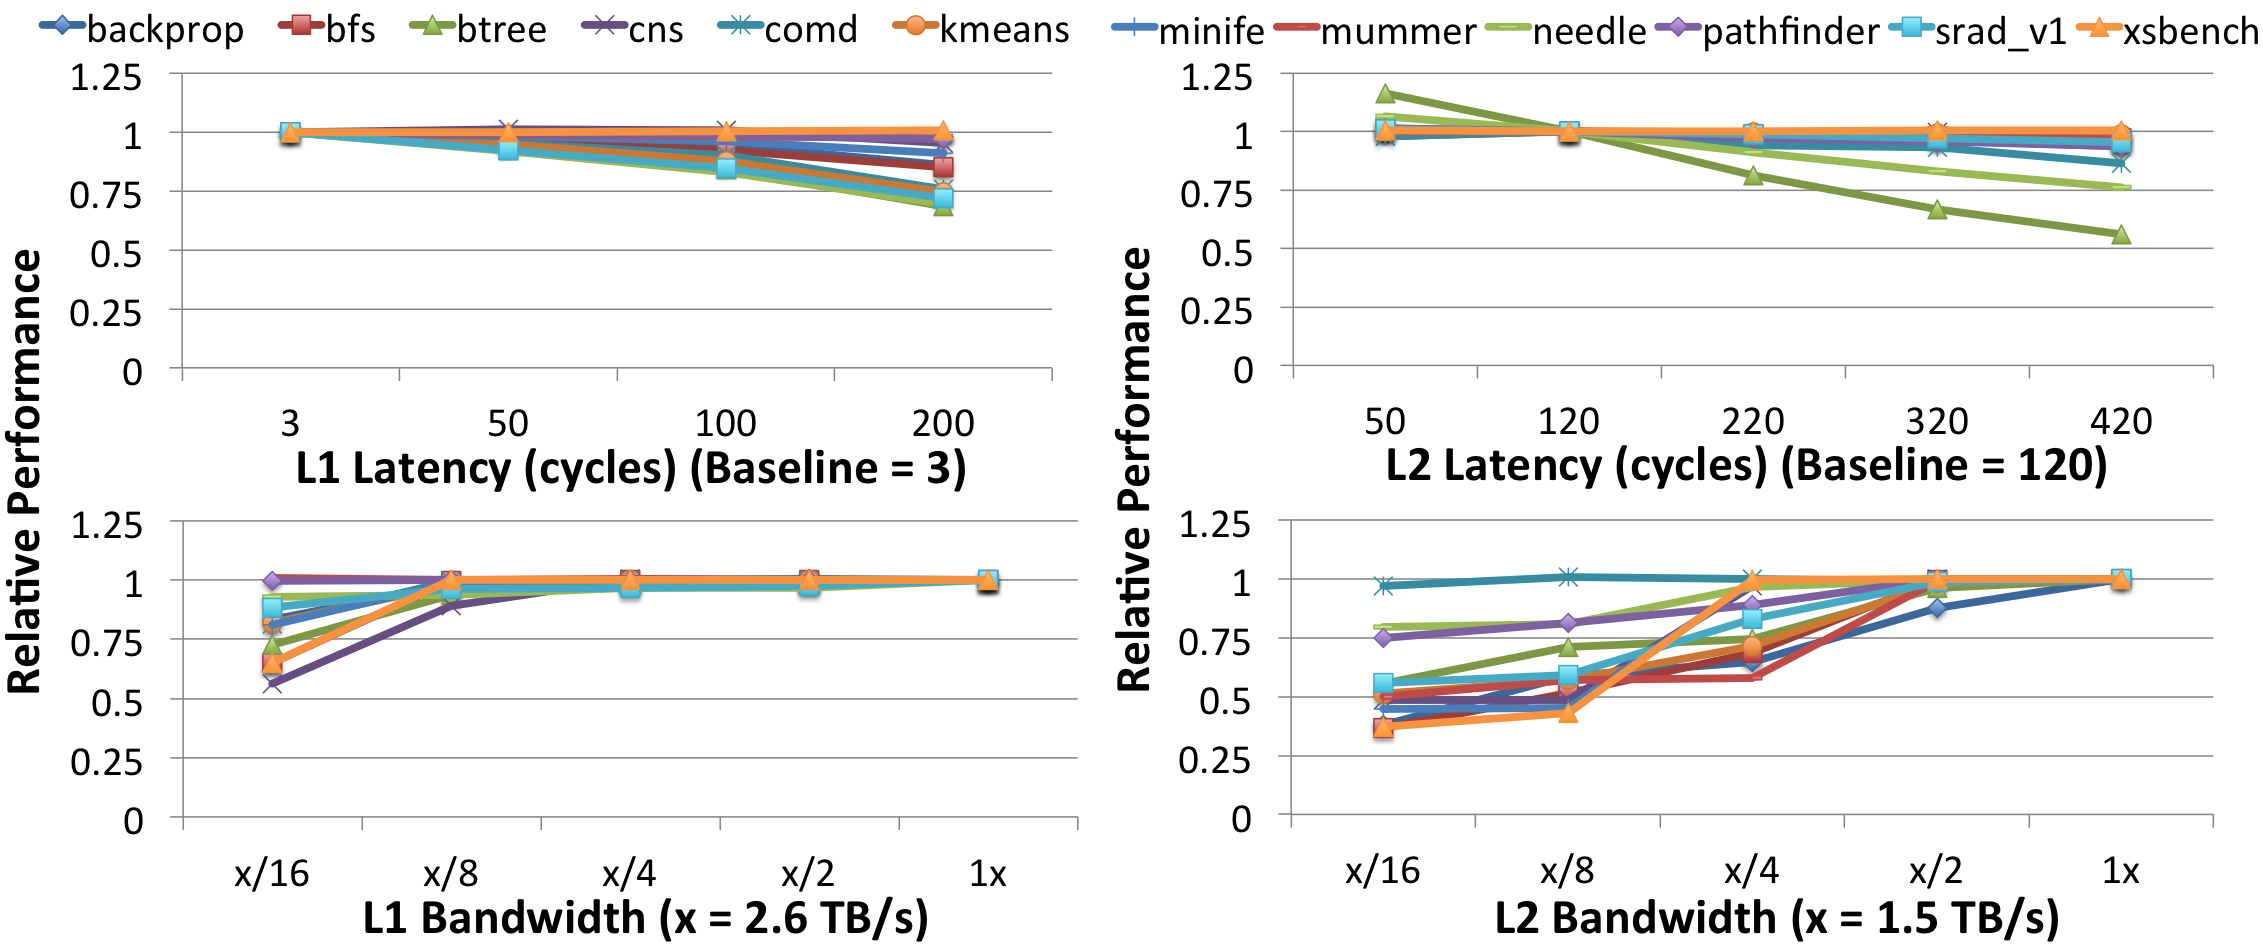
\includegraphics[width=\textwidth]{hpca2016/figures/cache_bw_latency.png}
    \caption{GPU performance sensitivity to L1 and L2 latency and bandwidth
changes.}
    \label{fig:cache_bw_latency}
    \vspace{-.1in}
\end{figure*}

As programming models supporting transparent CPU-GPU sharing become more
prevalent and sharing becomes more fine-grain and frequent, the performance gap
between page-level coherence and fine-grained hardware cache-coherent access
will grow~\cite{ref:agarwal:asplos2015,ref:agarwal:hpca2015,Lim2012}.  On-chip caches, and thus HW
cache coherence, are widely used in CPUs because they provide substantial memory
bandwidth and latency improvements~\cite{Martin2012}.  Building scalable,
high-performance cache coherence requires a holistic system that strikes a
balance between directory storage overhead, cache probe bandwidth, and
application
characteristics~\cite{Power2013,Pugsley2010,Cantin2005,johnson2011,Hong2012,Sanchez2012,Kelm2010}.
Although relaxed or scoped consistency models allow coherence operations to be
re-ordered or deferred, hiding latency, they do not obviate the need for HW
cache coherence. However, supporting a CPU-like HW coherence model in large
GPUs, where many applications do not require coherence, is a tax on GPU
designers.  Similarly, requiring CPUs to relax or change their HW coherence
implementations or implement instructions enabling software management of the
cache hierarchy adds significant system complexity.

Prior work has shown that due to their many threaded design, GPUs are
insensitive to off-package memory latency but very sensitive to off-chip memory
bandwidth~\cite{ref:agarwal:asplos2015,ref:agarwal:hpca2015}. Table~\ref{tab:gpuhitrate} shows the
L1 and L2 cache hit rates across a variety of workloads from the Rodinia and
United States Department of Energy application suites~\cite{Che2009,villa2014}.
These low hit rates cause GPUs to also be fairly insensitive to small changes in
L1 and L2 cache latency and bandwidth, as shown in
Figure~\ref{fig:cache_bw_latency}.  This lack of sensitivity raises the question
whether GPUs need to uniformly employ on-chip caching of all off-chip memory in
order to achieve good performance.  If GPUs do not need or can selectively
employ on-chip caching, then CPU--GPU systems can be built that present a
unified coherent shared memory address space to the CPU, while not requiring a
HW cache-coherence implementation within the GPU. 

Avoiding hardware cache coherence benefits GPUs by decoupling them from the
coherence protocol implemented within the CPU complex, enables simplified GPU
designs, and improves compatibility across future systems. It also reduces the
scaling load on the existing CPU coherence and directory structures by
eliminating the potential addition of hundreds of additional caches, all of
which may be sharing data. Selective caching does not come without a cost
however. Some portions of the global memory space will become un-cacheable
within the GPU\@ and bypassing on-chip caches can place additional load on
limited off-chip memory resources.  In the following sections, we show that by
leveraging memory request coalescing, small CPU-side caches, improved
interconnect efficiency, and promiscuous read-only caching, selective caching
GPUs can perform nearly as well as HW cache-coherent CPU--GPU\@ systems.

%}).\section{Background and Motivation}
%\label{motivation}
%
%\begin{figure}[t]
%\centering
%\includegraphics[width=1.0\columnwidth]{thermostat/figures/hotspot-cdf.png}
%\caption{HotSpot huge page distribution}
%\vspace{-0.175in}
%\label{fig:hotspot-cdf}
%\end{figure}
%
%Cold data at 4KB granularity vs 2MB granularity. Use figure to show quantify
%HotSpot pages within an otherwise cold huge page.
%
%Show analytical analysis of putting pages in slow memory and opportunity to make
%slow memory usable in data centers.
%
%Discuss performance-cost trade-off for data centers.
%
%Why are previous 2-level memory techniques inadeqaute in solving this issue.
%
%Re-iterate the problem we are solving and the central idea of our solution.
%
\section{Background}
\subsection{Virtual Memory Management}
\begin{figure}[t]
\centering
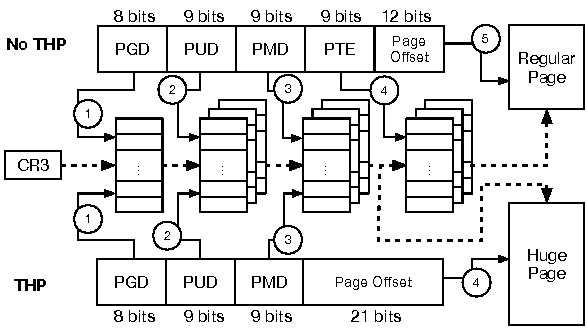
\includegraphics[width=0.45\textwidth]{thermostat/figures/linux_pgtable.pdf}
\caption{
Linux page table structure for X86 both with and without a transparent huge page.
}
\label{fig:linuxpgtable}
\end{figure}


As the size of main memory has grown, the overheads of virtual memory systems
have grown as well.  The hierarchical Linux page table for the x86-64
architecture, shown in Figure~\ref{fig:linuxpgtable}, addresses up to 128 terabytes of
memory and is four levels---and thus may incur up to four extra memory
operations to perform a single translation \cite{pgtable}.
%\fixme{This text is a candidate to cut to save space: Translation begins with
%the page global directory (PGD), pointed to by the CR3 register, which is
%preloaded with the PGD base address upon a context switch.  Bits 39-46 of the
%virtual address are used to index the PGD, yielding a page upper directory
%(PUD) structure, which is subsequently indexed by bits 30-38 of the virtual
%address to produce a page middle directory (PMD) structure.  When the
%translation target lies on a physical page of the 4 KB base page size (shown on
%the top in \pref{fig:linuxpgtable}), the PMD is indexed with bits 21-29, giving
%a page table entry (PTE) that is indexed by bits 12-20 to finally generate a
%physical page number.  Throughout this process, as many as four extra memory
%operations may be performed purely as an overhead of the virtual memory
%translation system.}
Moreover, execution in virtualized environments can sextuple translation costs
\cite{amdnested,intelept,bhargava:2008:atp}.  As a result, the Translation
Lookaside Buffer (TLB), which acts as a cache for virtual-to-physical mappings,
has become increasingly important to mollify the effects of virtual memory
translation overhead.

In most architectures, TLB accesses lie on the critical path of memory accesses,
hence hardware timing constraints limit the number of TLB entries that can be
searched on each access.  As memory capacities grow while page sizes remain
constant, TLB coverage---the portion of main memory that can be represented by
the contents of the TLB at any given time---necessarily decreases.  This reduced
coverage hampers the performance of programs with large working sets and/or
instruction footprints because it increases the number of TLB misses they
exhibit, and thus the number of page table walks that must be performed.  What's
more, as working set sizes---and, correspondingly, page table sizes---grow, the
fraction of translation data that can fit in the cache is reduced, leading to
more severe TLB miss penalties.

Recognizing the high cost of TLB misses in cloud applications, a number of
recent research efforts have sought hardware solutions to mitigate their penalty
(e.g., \cite{bhattacharjee:2011:slt, srikantaiah:2010:sth, barr:2011:sms,
pham:2012:ccl, basu:2013:evm, gandhi:2014:emv}.
Whereas these techniques reduce or hide TLB miss stalls, they do not address the
cost of managing numerous page tables entries or the cache capacity occupied by
them.

%One line of work seeks architectural solutions to improve the reach of TLBs,
%for example, through 2-level TLBs .  These mechanisms can improve TLB hit
%rates, but require hardware changes and do not address the cost of managing
%page tables, which manifest during a variety of system calls (e.g., upon
%allocations, faults to access \texttt{mmap()}'d files, and forks).  A second
%line of work revisits alternative memory virtualization schemes, such as
%segmentation, in the context of modern systems \cite{basu:2013:evm,
%gandhi:2014:emv}.  While new hardware support for segmentation may address TLB
%capacity limitations for the user heap, it does not provide a straightforward
%solution for OS structures that may require finer-grained protection, such as
%the file system page cache.

Huge pages directly address the costs of fine-grain page management.
%They require hardware support in the TLB for huge-page entries (either
%dedicated entries or support for multiple-sized lookups), but this support is
%ubiquitous in existing architectures (e.g., Intel's Haswell processor
%provisions 32 entries for huge pages in its L1 data TLBs).
They effectively increase TLB coverage---one huge page TLB entry covers the area
of a large number of regular page entries---thus reducing page faults, and they
reduce the size of the page table structure, leading to both fewer memory
accesses upon a TLB miss and increased cache-ability of translation data.
%on a TLB miss they can reduce the number of page table accesses necessary to
%resolve a virtual-to-physical mapping.  The latter arises due to the fact that
%a huge page covers a much larger range of virtual memory.
%\pref{fig:ahppgtable} displays the most efficient possible hierarchical page
%table topology for x86-64 Linux if it is backed by 2MB huge pages.
%In contrast to the page table shown in \pref{fig:linuxpgtable}, this structure
%requires only two extra memory accesses due to the increased coverage at each
%level.  Though TLB support for huge pages is ubiquitous in existing
%architectures (e.g., Intel's Haswell processor TLBs provision 32 entries for
%huge pages in the L1 data TLB), unfortunately the current x86-64 architecture
%specifies the page table layouts shown in \pref{fig:linuxpgtable}.
%and precludes a design like that in \pref{fig:ahppgtable}.
%We hope our results might motivate greater flexibility in future architecture
%revisions.
%
%\input{fig.ahppgtable}

\subsection{Background: Transparent Huge Pages} \label{sec:thp_bg}
%\fixme{This paragraph strongly duplicates the intro.  We should say this in
%only one place.  My suggestion is to cut down the intro and leave the details
%here. --- Jeff: fixed}
Early system support for huge pages, static huge pages, requires bucketing the
available physical memory at boot time into standard pages and huge pages.
Static huge pages are disjoint from the standard memory pool and cannot be used
for the disk page cache, disk write buffers, or any kernel data structure.
Moreover static huge pages require application changes and are thus
non-transparent to the programmer. The static provisioning of memory into static
huge pages also leads to allocation problems and memory stranding if the actual
demand for huge pages does not match the boot-time configuration.  Thus, even if
applications are static huge page-aware, such a solution is less than ideal for
many systems because it requires a priori knowledge of applications' memory
requirements to ensure ideal performance.

Recent versions of the Linux kernel instead exploit huge pages through THP.
With THP, the kernel attempts to invisibly (i.e., without the knowledge of the
user) allocate huge pages to back large regions of contiguous virtual memory.
Transparent allocation is advantageous because it allows existing codebases to
reap the rewards of huge pages without modification and doesn't require changing
the interfaces and invariants of system calls and functions that require
consideration of page size, such as \texttt{mmap()}.  However, the kernel may
demote allocated huge pages by breaking them down into a set of regular pages
when it deems necessary  to maintain support for functions that are not huge
page-aware.

\textbf{Allocation/Promotion:} The first time an application touches an
allocated region of virtual memory, a page fault occurs and the kernel allocates
one or more physical pages to back that region and records the virtual to
physical mapping.  With THP enabled, the kernel allocates huge pages for
anonymous (i.e., non-file-backed) regions of huge page-sized and -aligned
virtually contiguous memory during the initial page fault to that region.
%Alternatively, if a huge page isn't initially available or the size and
%alignment requirements are not met, a region of virtual memory that isn't
%initially backed by huge pages can later be promoted if the virtual region is
%later modified to meet these requirements.  In the process of promotion, the
%regular page-backed virtual region is collapsed into a huge page-backed region,
%thus multiple regular pages are marked to be treated as a single huge page.
Alternatively, if a region isn't initially backed by a huge page, it can later
undergo promotion, in which multiple regular pages are marked to be treated as a
single huge page.  The kernel can be set to either aggressively allocate huge
pages whenever it can, or to only allocate them when the user provides hints via
the \texttt{madvise()} system call.

\textbf{Demotion:} Any region backed by a huge page may be subject to
spontaneous demotion to regular pages.  Because various parts of the kernel
source code are not huge page-aware, giving them access to a huge page could
lead to unspecified or erroneous behavior.  As a result, huge pages are often
\emph{split}, or broken into several regular pages, before they are passed to
functions that are not huge page-aware.  To perform this split, the page table
must be updated to reflect the many regular pages that comprise the demoted huge
page.

%Another notable characteristic of THP is that it does not increase the coverage
%of the various levels of the page table (due to architectural constraints
%described in \pref{sec:limitations}).  Therefore, while the physical page size
%is increased, the coverage of each level of the page table remains the same.
%The translation procedure for \thp, shown on the bottom in
%\pref{fig:linuxpgtable}, elides the PMD$\to$PTE step necessary with regular
%pages and produces a physical page number at the PMD level.
%
%In contrast to the two memory access translation shown in
%\pref{fig:ahppgtable}, a \thp translation requires three accesses.
%
%\subsection{Pathologies of THP} \label{sec:thp_problems}
%
%\input{fig.frag_bench.tex}
%
%Though \thp has the potential to improve average application throughput, it can
%negatively impact latency and performance isolation between unrelated
%applications.  A widely known effect of paged virtual memory is external memory
%fragmentation---small blocks of free memory separated by large blocks of
%allocated memory.  With \thp, a system exhibiting significant memory
%fragmentation may not always have huge page-sized regions of contiguous
%physical memory available for allocation, even if much of memory is free.
%
%Severe memory fragmentation is particularly common in cloud computing
%workloads, where processes start and end frequently.  In systems with few,
%long-lived processes, virtual memory rarely becomes fragmented---most user-mode
%allocators do not frequently return freed memory to the operating system,
%instead retaining and managing it in pools.  In contrast, many cloud
%environments collocate multiple processes that start and end frequently in a
%single machine.  For example, map-reduce clusters execute thousands of
%processes that may each last only minutes.  Main memory will rapidly fragment
%due to the varying allocation sizes of these numerous short-lived processes.
%I/O intensive workloads can also cause rapid memory fragmentation due to random
%access I/O populating the page cache with many small allocations, which are
%subsequently reclaimed without regard to layout.
%
%When a huge page is requested during a page fault but cannot be served, the
%Linux memory manager has two options: it can either turn down the request and
%fall back on regular pages to serve the fault, or it can stall the program and
%defragment memory to create a huge page-sized chunk to allocate.  The former
%option is not ideal, as it prevents applications from reaping the benefits of
%huge pages when there is still enough physical memory available to accommodate
%them.  However, the performance cost of synchronous (\ie, blocking)
%defragmentation can be significant, as execution of the application must be
%paused while the kernel migrates regular pages to make room for a huge page.
%
%While defragmentation is in progress, the kernel will obtain and hold locks
%that can block progress of other applications that happen to concurrently
%request memory.  Hence, defragmentation impacts not only the application
%requesting the huge page, it can also result in stalls in ``innocent
%bystander'' applications.  Indeed, in our experience, a pathological behavior
%in defragmentation code triggered by one application caused multi-millisecond
%(and initially unexplainable) latency spikes in an unrelated production service
%that happened to collocate on the same server.  The kernel locks held by
%defragmentation code caused allocation delays to spread virally among
%applications.  These THP pathologies have been documented by others as well
%\cite{zhuang:2014:ehm, rientjes:2014:email, oracle:2013:blog, rahn:2012:blog}.
%Whereas some of these issues have been mitigated (after several man-months of
%investigation), these pathologies motivated this study of the \thp mechanism,
%and prompted us to ask whether, perhaps, the entire mechanism should be
%discarded.
%
%To our dismay, one such pathology in \thp can be triggered in recent versions
%of the kernel (in which the behavior is ostensibly fixed), even without exotic
%application behaviors.  To reconstruct this behavior, we use a memory
%allocation microbenchmark that measures the latency of allocation (\ie, time
%needed for the kernel to find and map a physical page) for 2MB regions
%allocated on the heap using unmodified GLIBC \texttt{malloc()}.
%\pref{fig:frag_bench} shows the impact of synchronous memory defragmentation on
%allocation tail latency in a virtual machine running version 3.13 of the Linux
%kernel.
%% when using only \texttt{malloc()} to fragment memory, as might naturally arise after running map-reduce processes for several hours. %
%%We measure a memory allocation microbenchmark, which allocates and initializes huge page-sized chunks of memory using unmodified GLIBC \texttt{malloc()}, causing the kernel to attempt to allocate huge pages when the THP mechanism is enabled.
%We report the cumulative distribution of the latency of individual allocations
%(note the logarithmic x-axis scale).  We consider four scenarios, two with \thp
%enabled and two with it disabled.  We consider scenarios where memory is
%initially unfragmented (all memory is free and the page cache is empty) and
%where it has been aggressively fragmented.  We fragment memory using a large
%number of processes that repeatedly allocate and free memory chunks of random
%sizes---a scenario representative of a series of map-reduce tasks.  These
%processes are continually spawned and killed (to return their allocated memory
%to the kernel), with the last set of processes ultimately holding a final set
%of allocations (partially filling memory) and quiescing.  Further details of
%our test setup appear in \pref{sec:methodology}. %\fixme{Confirm that we
%actually do provide further details in the results section.}
%
%There are two key take-aways from this experiment.  First, \thp substantially
%reduces latency for most allocations.  Median allocation latency is reduced
%from about 700us to about 500us.  Allocations become faster on average because
%the kernel must create and map far fewer PTEs (by as much as a factor of 512)
%for large allocations.  When memory is unfragmented, nearly all allocations are
%faster under \thp.  In contrast, when memory is fragmented, synchronous
%compaction severely delays a significant fraction of allocations, in some cases
%increasing latency by orders of magnitude.  About 20\% of allocation requests
%take longer than 1ms with allocations in the 99th percentile taking over 100ms.
%
%Though the tail latency of memory allocation under such circumstances isn't
%critical in all applications, especially those with steady-state heap activity,
%it can have negative effects on other tail-latency-sensitive workloads.
%Workloads such as web search, for instance, perform significant fan-out and
%fan-in operations, where stragglers impact overall latency
%\cite{dean:2013:tas}.  For such applications, unpredictable allocation tail
%latency or stalls of bystander applications/threads can severely impact
%application service level objectives.
%
%One alternative to avoid this unpredictability is to asynchronously (\ie, on
%idle cores) defragment memory to help alleviate the amount of defragmentation
%that must be done at allocation time.  This feature is available in the Linux
%kernel, but it comes with a tradeoff: setting the defragmentation daemon to be
%too aggressive causes it to consume substantial CPU time, harming the
%performance of other threads (and reducing the throughput benefit of \thp)
%\cite{zhuang:2014:ehm}, but setting it to be too passive results in little net
%benefit.  We examine this trade-off in \pref{sec:case_study}.  Alternatively,
%one might reduce the aggressiveness of or disable synchronous compaction
%altogether.  However, doing so often precludes huge page allocation, resulting
%in a performance loss in the common cases where synchronous defragmentation
%does not dominate allocation time.  Thus, supporting multiple pages sizes leads
%to a catch-22; aggressive compaction leads to performance loss due to invasive
%use of system resources, and less aggressive or no compaction results in
%performance loss because huge pages cannot always be allocated on-demand.  As a
%result, THP---or any system that supports multiple page sizes---is inherently
%disadvantaged when large chunks of memory are scarce, as when the system is
%under heavy memory pressure or subject to external fragmentation.
%%
%%under memory pressure or fragmentation.

